\begin{sidewaysfigure*}
\begin{center}
\rotatebox{90}{~~~~~~Small Resource Wave}
\hspace{1ex}
\begin{subfigure}[b]{0.1825\linewidth}
  \centering
  Mutational Load 1\\~\\
  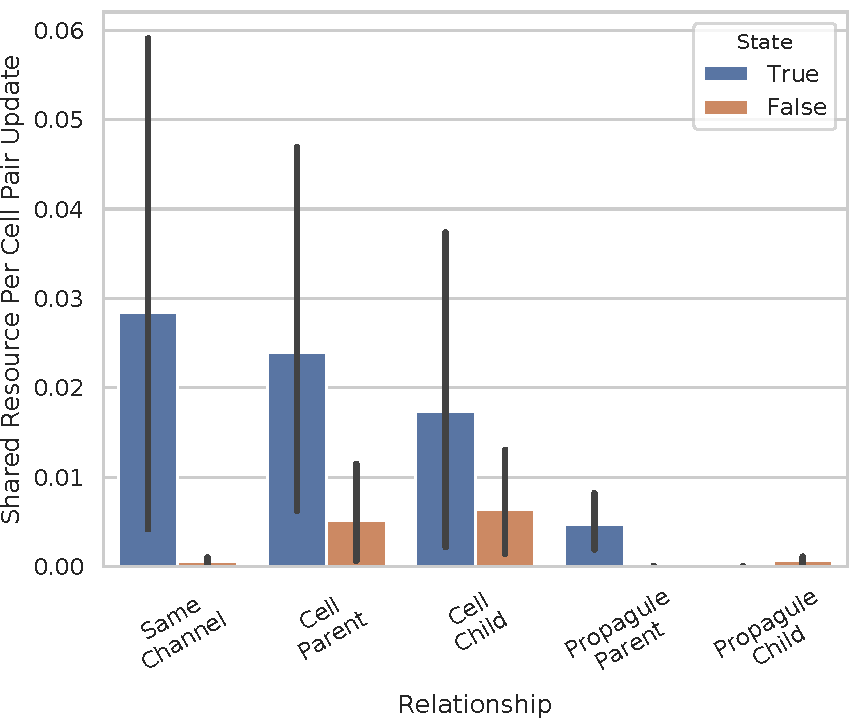
\includegraphics[width=\linewidth]{title=resource_contributed+treat=wave-small__mut-a_low+_data_hathash_hash=e071a43082c10cd4+_script_fullcat_hash=064800f3ddff6753+_source_hash=d53f428-clean+ext=}
\end{subfigure}
\hspace{1ex}
\begin{subfigure}[b]{0.1825\linewidth}
  \centering
  Mutational Load 2\\~\\
  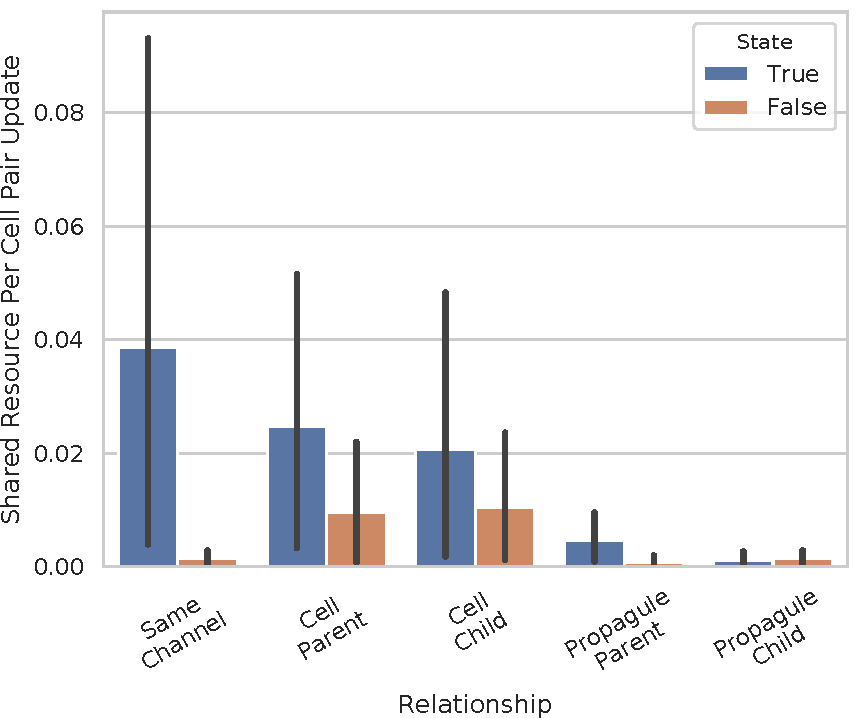
\includegraphics[width=\linewidth]{title=resource_contributed+treat=wave-small__mut-b_medlow+_data_hathash_hash=b470f6e885f49798+_script_fullcat_hash=064800f3ddff6753+_source_hash=d53f428-clean+ext=}
\end{subfigure}
\hspace{1ex}
\begin{subfigure}[b]{0.1825\linewidth}
  \centering
  Mutational Load 3\\~\\
  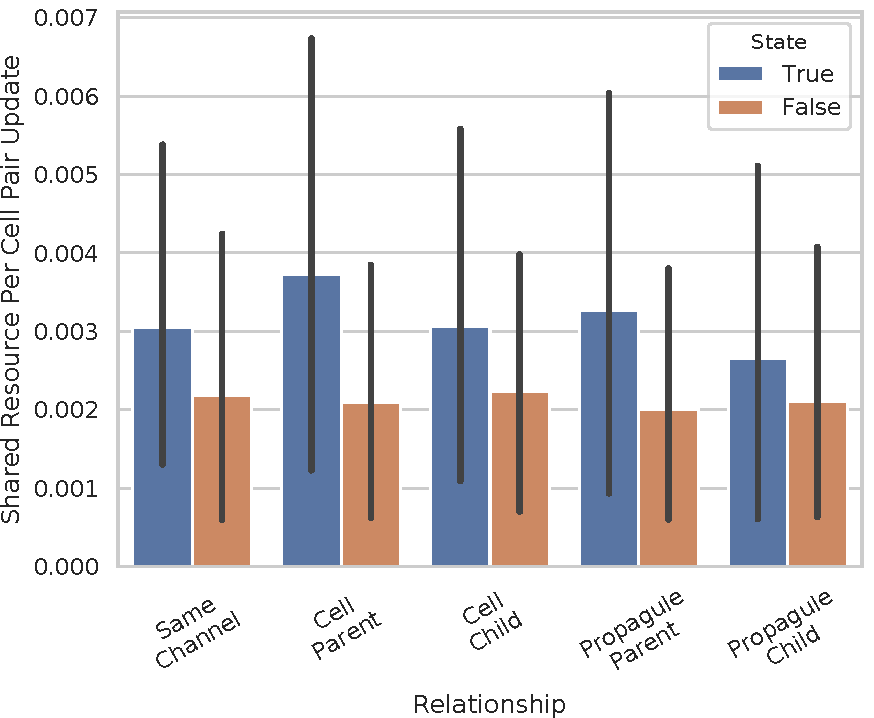
\includegraphics[width=\linewidth]{title=resource_contributed+treat=wave-small__mut-c_medhigh+_data_hathash_hash=09904fe0c4f292cc+_script_fullcat_hash=064800f3ddff6753+_source_hash=d53f428-clean+ext=}
\end{subfigure}
\hspace{1ex}
\begin{subfigure}[b]{0.1825\linewidth}
  \centering
  Mutational Load 4\\~\\
  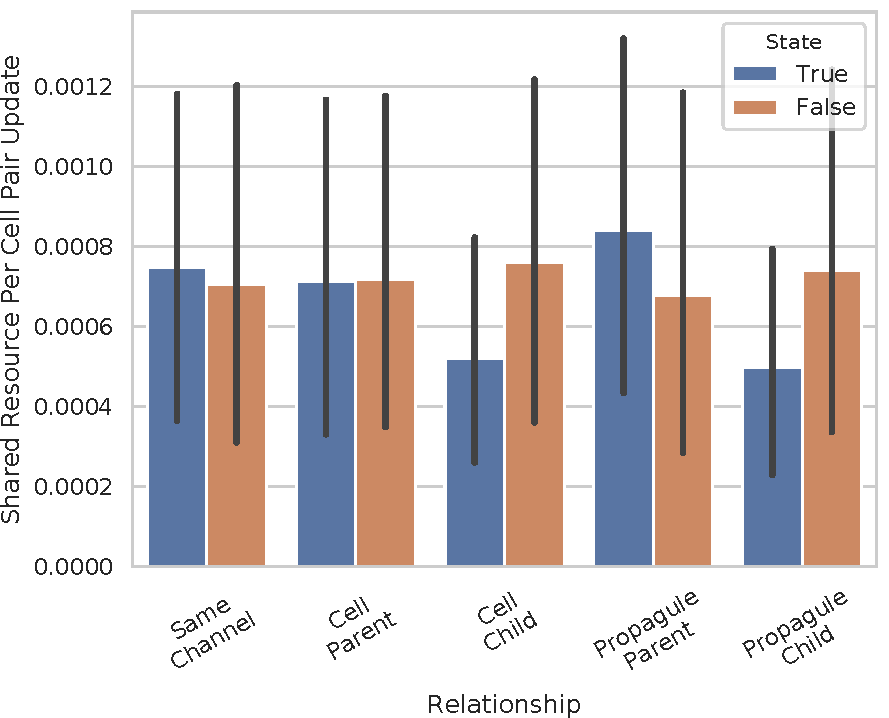
\includegraphics[width=\linewidth]{title=resource_contributed+treat=wave-small__mut-d_high+_data_hathash_hash=0508b355e6755132+_script_fullcat_hash=064800f3ddff6753+_source_hash=d53f428-clean+ext=}
\end{subfigure}
\hspace{1ex}
\begin{subfigure}[b]{0.1825\linewidth}
  \centering
  Mutational Load 5\\~\\
  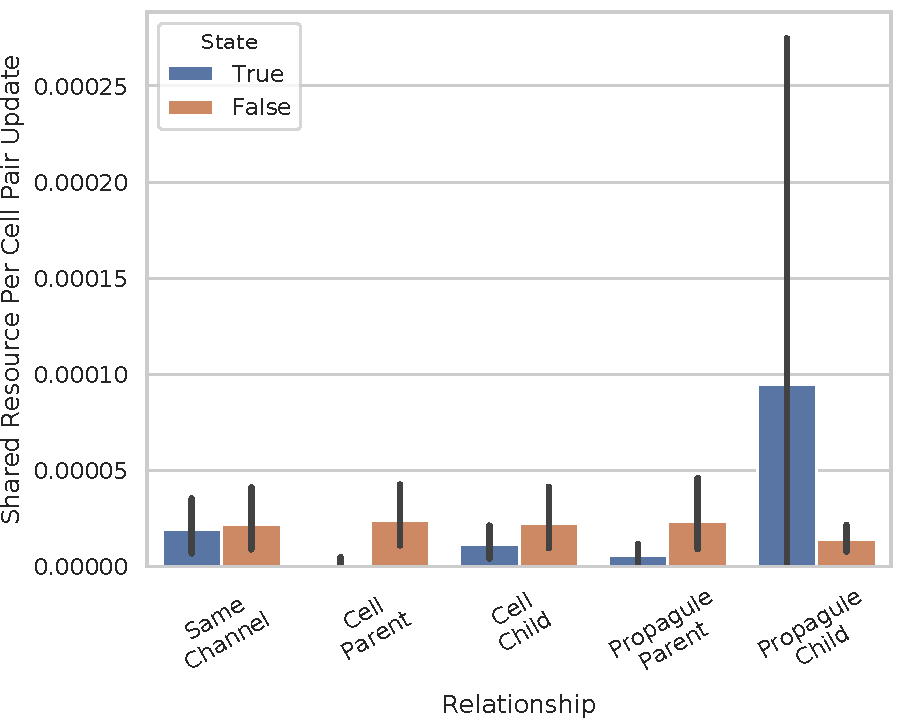
\includegraphics[width=\linewidth]{title=resource_contributed+treat=wave-small__mut-e_extreme+_data_hathash_hash=0b12a3f7b0d9143b+_script_fullcat_hash=064800f3ddff6753+_source_hash=d53f428-clean+ext=}
\end{subfigure}\\
\vspace{5ex}

\rotatebox{90}{~~~~~~Large Resource Wave}
\hspace{1ex}
\begin{subfigure}[b]{0.1825\linewidth}
  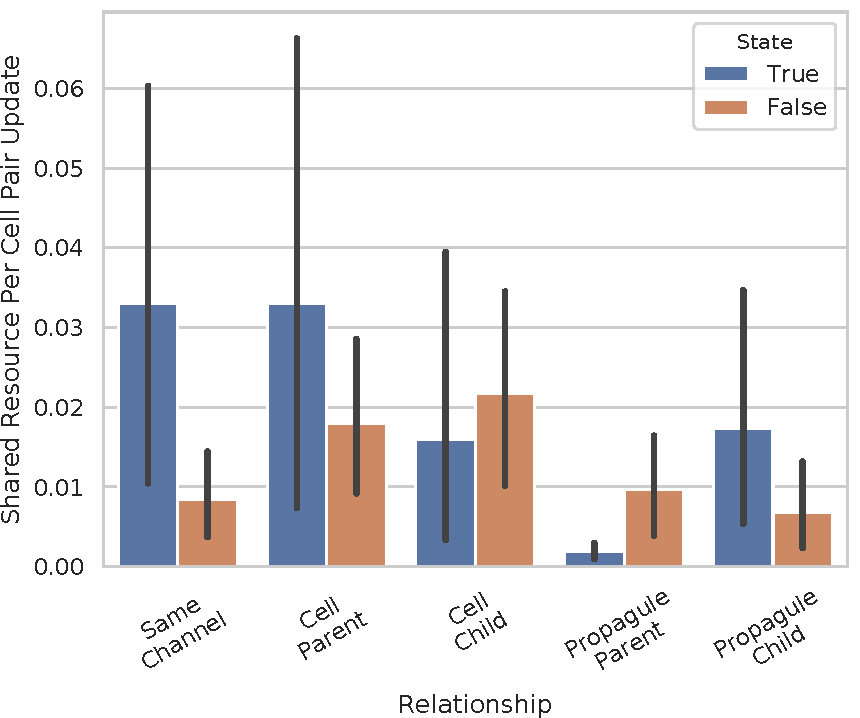
\includegraphics[width=\linewidth]{title=resource_contributed+treat=wave-big__mut-a_low+_data_hathash_hash=0687f354f3d94aaa+_script_fullcat_hash=064800f3ddff6753+_source_hash=d53f428-clean+ext=}
\end{subfigure}
\hspace{1ex}
\begin{subfigure}[b]{0.1825\linewidth}
  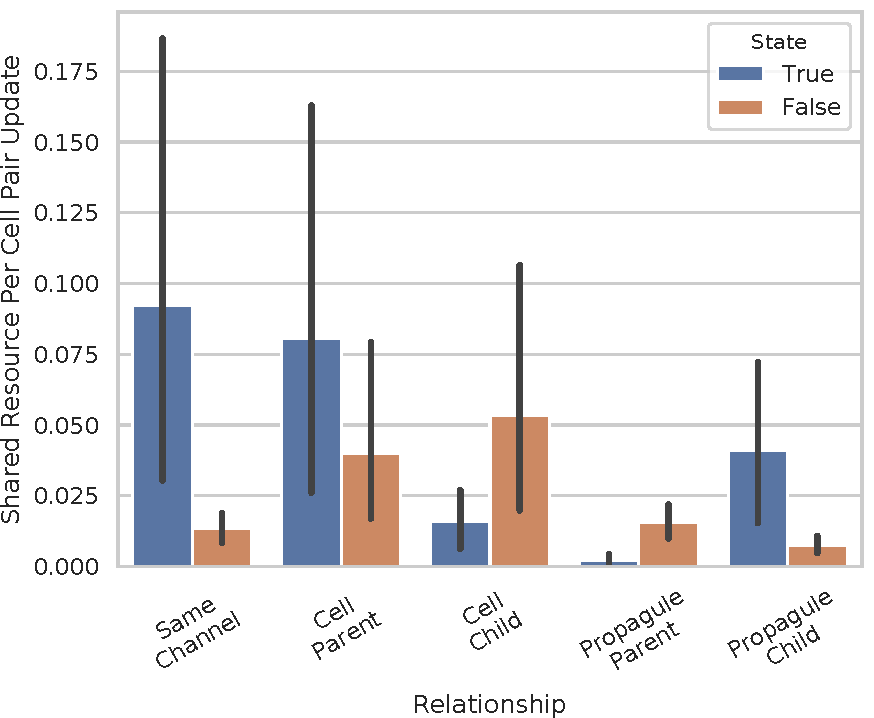
\includegraphics[width=\linewidth]{title=resource_contributed+treat=wave-big__mut-b_medlow+_data_hathash_hash=91d8a5c7499340cf+_script_fullcat_hash=064800f3ddff6753+_source_hash=d53f428-clean+ext=}
\end{subfigure}
\hspace{1ex}
\begin{subfigure}[b]{0.1825\linewidth}
  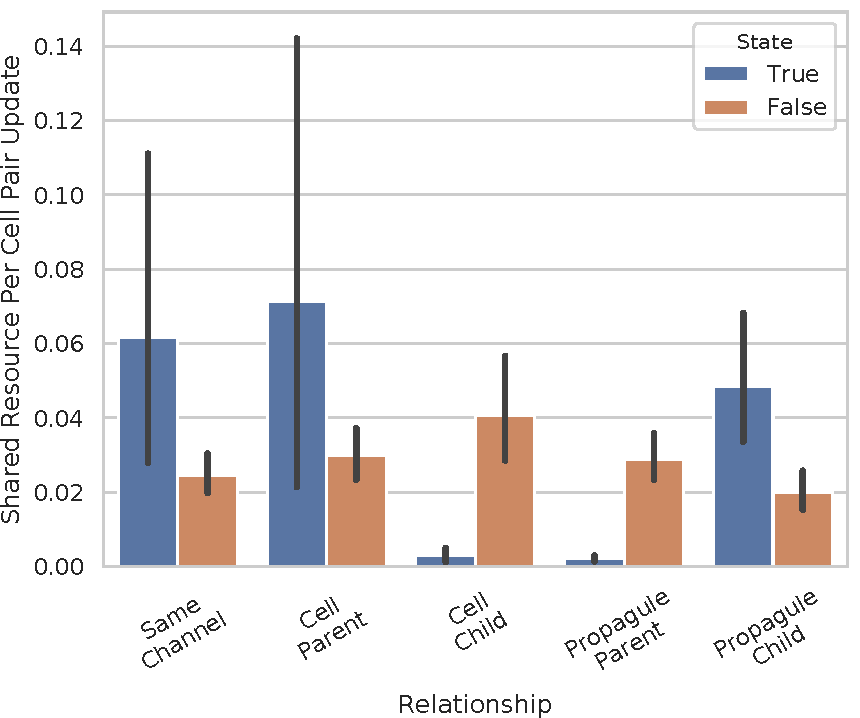
\includegraphics[width=\linewidth]{title=resource_contributed+treat=wave-big__mut-c_medhigh+_data_hathash_hash=9046a546605ce7d0+_script_fullcat_hash=064800f3ddff6753+_source_hash=d53f428-clean+ext=}
\end{subfigure}
\hspace{1ex}
\begin{subfigure}[b]{0.1825\linewidth}
  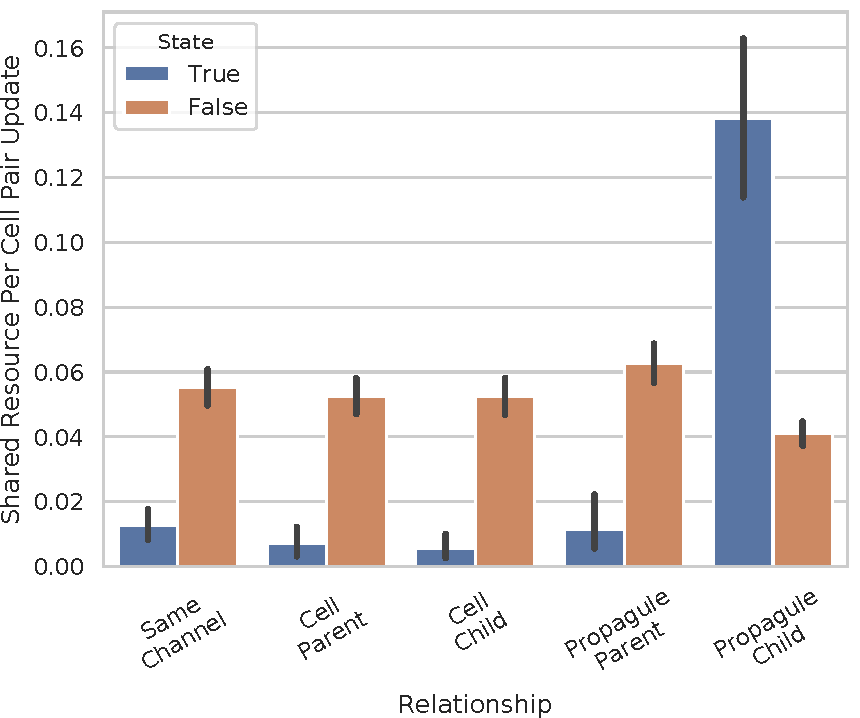
\includegraphics[width=\linewidth]{title=resource_contributed+treat=wave-big__mut-d_high+_data_hathash_hash=8c358ba0aef47998+_script_fullcat_hash=064800f3ddff6753+_source_hash=d53f428-clean+ext=}
\end{subfigure}
\hspace{1ex}
\begin{subfigure}[b]{0.1825\linewidth}
  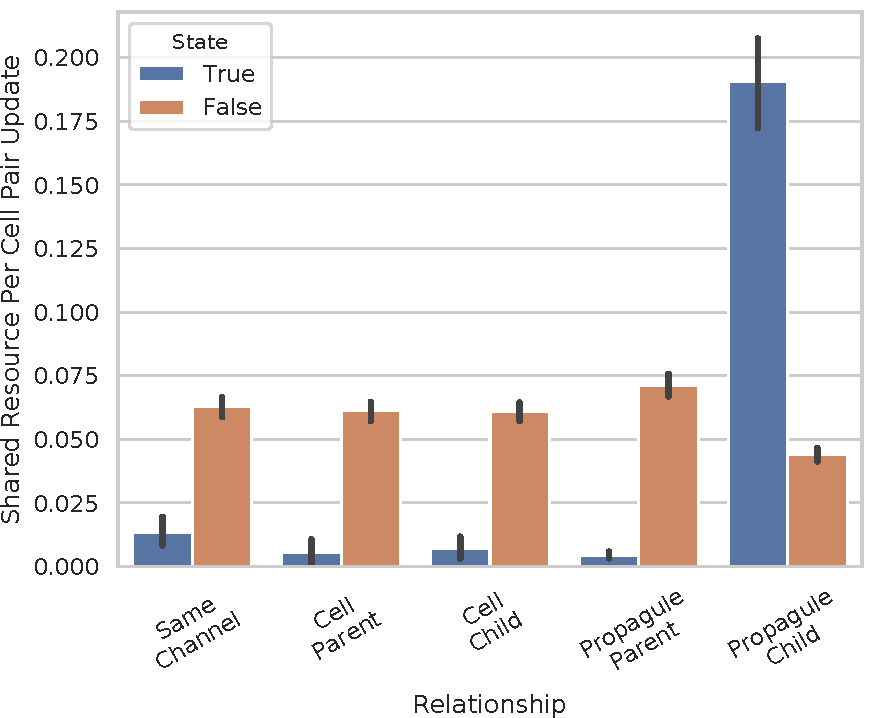
\includegraphics[width=\linewidth]{title=resource_contributed+treat=wave-big__mut-e_extreme+_data_hathash_hash=5e17f0d9addba523+_script_fullcat_hash=064800f3ddff6753+_source_hash=d53f428-clean+ext=}
\end{subfigure}\\
\vspace{5ex}
\caption{
Detailed audits of resource sharing phenotypes by treatment.
Bar height represents the mean amount of resource transferred per update per neighboring pair of cells.
Each two-tone pair of bars compares cell pairs with a particular relationship to cell pairs without that relationship.
The ``Same Channel'' bar pair compares resource sharing between cell pairs with a common channel and cell pairs on different channels.
The ``Cell Parent'' bar pair compares the amount of resource shared from a cell to its cellular parent to the amount of resource shared from a cell to cells that are not its cellular parent.
The ``Cell Child'' bar pair compares the amount of resource shared from a cell to its cellular child to the amount of resource shared from a cell to cells that are not its cellular child.
For the next two relationships, consider a cell with channel ID $A$ that reproduces, producing a daughter cell with the new channel ID $B$.
Let the channel ID $C$ denote a channel ID that is unique from channel IDs $A$ and $B$.
The ``Propagule Parent'' bar pair compares the amount of resource shared from a cell to cells with the channel ID that its channel ID descends from (e.g., from cells with channel ID $B$ to cells with channel ID $A$) to the amount of resource shared to other cells that are not part of its same-channel network (e.g., to cells with channel ID $C$).
The ``Propagule Child'' bar pair compares the amount of resource shared from a cell to cells with a channel ID that descends from its channel ID (e.g., from cells with channel ID $A$ to cells with channel ID $B$) to the amount of resource shared to other cells that are not part of its same-channel network (e.g., to cells with channel ID $C$).
Error bars represent 95\% confidence intervals.
}
\label{fig:resource_contributed_by_treat}
\end{center}
\end{sidewaysfigure*}
